% !TeX root = ../../main.tex
\section{Miary skuteczności sieci}

W kolejnych rozdziałach, na potrzeby oceny skuteczności sieci neuronowej, dla danego obrazu i przewidzianej przez sieć maski, każdy piksel można zaklasyfikować do jednej z następujących kategorii:

\begin{itemize}
  \item True Positive - piksel został poprawnie zakwalifikowany jako powierzchnia kortu;
  \item False Positive - piksel nie wchodzący w powierzchnię kortu został niepoprawnie oznaczony jako powierzchnia kortu;
  \item False Negative - piksel kortu został niepoprawnie zakwalifikowany jako nie wchodzący w powierzchnię kortu;
  \item True Negative - piksel został poprawnie zakwalifikowany jako nie wchodzący w powierzchnię kortu.
\end{itemize}

W przypadku zbioru \textit{low} wszystkie obrazy w tym zbiorze są tej samej rozdzielczości 896x640 pikseli, a co za tym idzie każdy składa się z identycznej liczby pikseli w sumie.
Korzystając z tego faktu, testując sieć na elementach zbioru \textit{low} wyniki powyższej klasyfikacji można w miarodajny sposób uśredniać między różnymi obrazami.

\begin{figure}[!htb]
  \minipage{0.45\textwidth}
    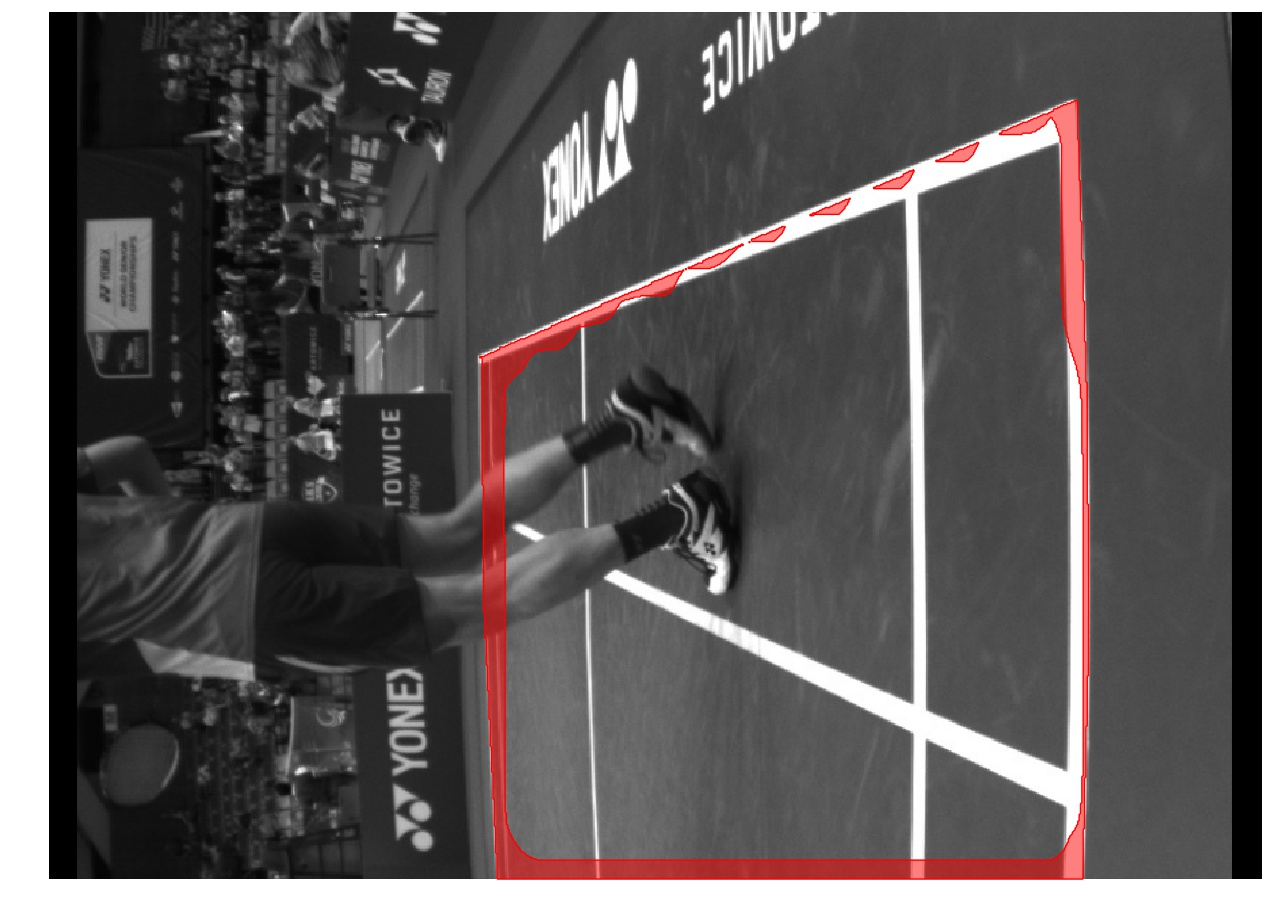
\includegraphics[width=\linewidth]{original_fn_1564911595553287247.jpg}
    \caption{Poglądowy obraz z zaznaczonym obszarem False Negative}
  \endminipage\hfill
  \minipage{0.45\textwidth}
    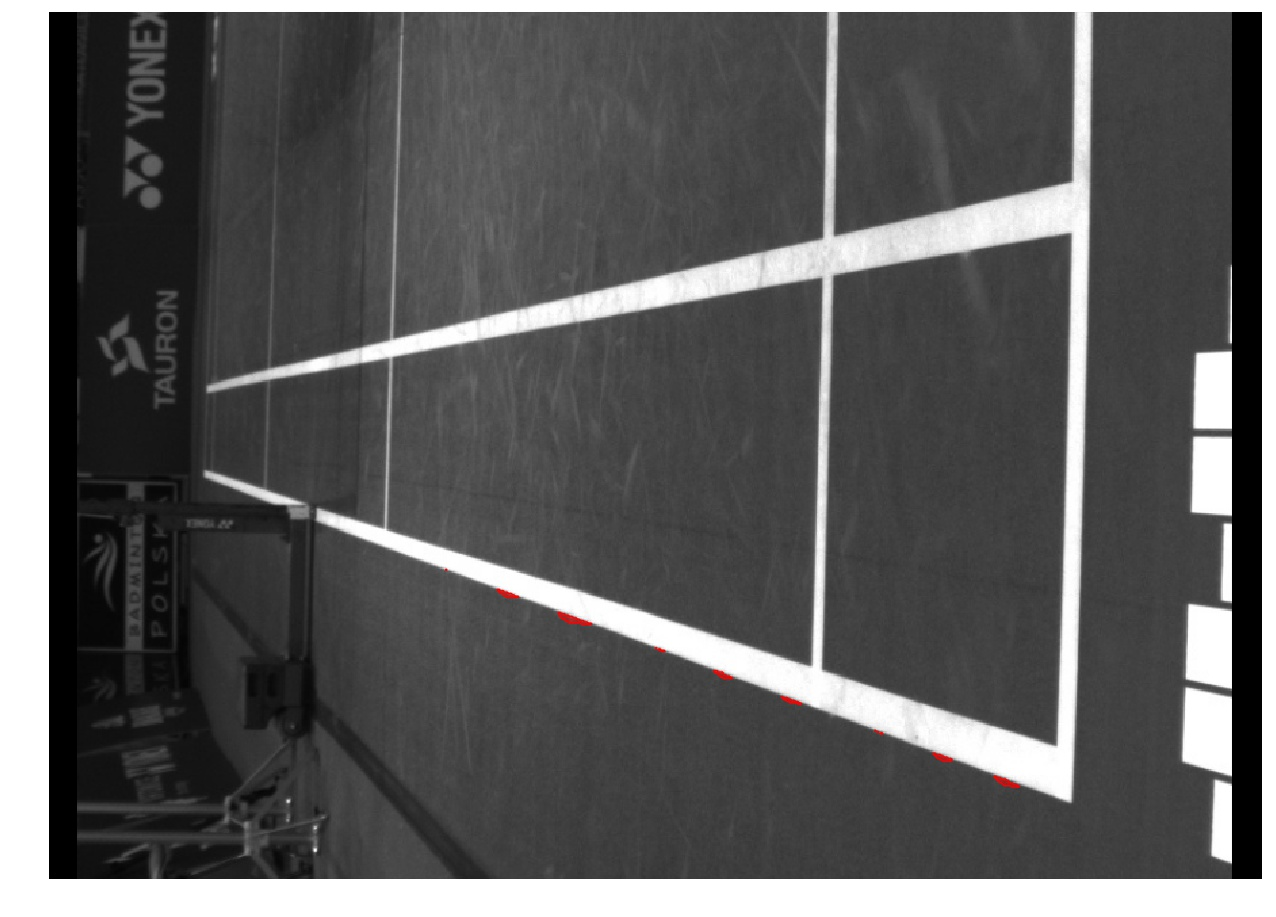
\includegraphics[width=\linewidth]{original_fp_1564953159296706208_5.jpg}
    \caption{Poglądowy obraz z zaznaczonym obszarem False Positive}
  \endminipage\hfill
\end{figure}

Znając klasyfikację pikseli na obrazach, można obliczyć następujące, bardziej złożone metryki:

\begin{itemize}
  \label{sec:miary}
  \item Accuracy - $ \frac{TP + TN}{TP + TN + FP + FN} $,
  \item Sensitivity - $ \frac{TP}{TP + FN} $,
  \item Specificity - $ \frac{TN}{TN + FP} $,
  \item Precision - $ \frac{TP}{TP + FP} $;
\end{itemize}

Kolejne rozdziały zawierają wyliczenia powyższych metryk, z których za najistotniejszą przyjęto \textit{Accuracy} uśrednioną na testowanym zbiorze danych, ponieważ można ją porównać ze skutecznością algorytmu wykorzystywanego w firmie \blue{}.
